\section{Compound DMA \DIFdelbegin \DIFdel{attacks}\DIFdelend \DIFaddbegin \DIFadd{Attacks}\DIFaddend }\label{sec:linux_net}

%\adam{This section is significantly less organized than the rest of the paper (the fact you discuss IOTLB in two places is an example. I suggest to organize it according to the characterizations: first explain how the networking system design makes the 3/4 vulnerability types occur, then have sections according to the trifecta where you explain how those are obtained, and title them accordingly, not with cute but not meaningful names. Following my comment about the 3rd ``sub-page'' vuln type (multiple mapping), which doesn't belong as a vuln type, I suggest introducing that here (since really, this is what's happening anyway).}

%\adam{I'd retitle this section: it is about kernel design flaws to enable getting Motive, Means, and Opportunity}

%So far, we have demonstrated a \simple attack by exploiting type (a) \subpage vulnerability of the FireWire driver. 
This section explores new attacks on the Linux network stack\DIFaddbegin \DIFadd{, }\DIFaddend where the vulnerability attributes are initially missing but are attainable via compound steps.
We focus on the Linux network stack\DIFdelbegin \DIFdel{which initially seems }\DIFdelend \DIFaddbegin \DIFadd{, which initially appears  }\DIFaddend secure~\cite{thunder}.
Nevertheless, as we demonstrate, the Linux network stack is actually responsible for 60\% of the DMA vulnerabilities \mbox{we \DIFdelbegin \DIFdel{have }\DIFdelend found.}

Recall that, once we have discovered a \subpage{} vulnerability, our goal is to obtain the three vulnerability attributes \DIFdelbegin \DIFdel{(Sec. }\DIFdelend \DIFaddbegin \DIFadd{described in Section }\DIFaddend \ref{sec:mmo}: (1) a KVA, (2) a callback pointer and, (3) timing\DIFdelbegin \DIFdel{)}\DIFdelend . 
Accordingly, in \DIFdelbegin \DIFdel{Sec.}\DIFdelend \DIFaddbegin \DIFadd{Section}\DIFaddend ~\ref{sec:shinfo_exploit}, we first describe how to obtain (2) a callback function pointer. Then, in \DIFdelbegin \DIFdel{Sec.}\DIFdelend \DIFaddbegin \DIFadd{Section}\DIFaddend ~\ref{sec:timely}, we show that (3) a time window for exploiting this pointer is available. 
While these two steps for obtaining vulnerability attributes (2) and (3) are generic, there are different recipes for how to obtain the remaining vulnerability attribute (1), i.e., the KVA of the malicious buffer.
We complete the vulnerability attributes in \DIFdelbegin \DIFdel{Sec.}\DIFdelend \DIFaddbegin \DIFadd{Section}\DIFaddend ~\ref{sec:ringflod}, \DIFdelbegin \DIFdel{Sec.~\ref{sec:posion}and Sec.~\ref{appx:additional_compound}}\DIFdelend \DIFaddbegin \DIFadd{Section~\ref{sec:posion}, and Section~\ref{appx:additional_compound}, }\DIFaddend by showing different ways \DIFdelbegin \DIFdel{(by which we also name the compound attack) }\DIFdelend \mbox{to obtain (1) the KVA.}



%Due to space limitations we demonstrate only selected compound DMA attacks. 
%Upon the publication of our work, we aim to release extended material, including evaluation scripts and additional \compound and previously unknown \simple attacks found by our tools.
%\sout{We first describe the vulnerable data structures shared by \emph{all} Linux network drivers, which exposes a callback pointer. Then, after providing some necessary technical background (Sec.~\ref{sec:deferred}), we show how that the device is often provided with a timing window during which a modified callback pointer will be executed by the CPU~(Sec.~\ref{sec:shinfo}). Finally, we discuss various methods to identify kernel virtual addresses of pages containing malicious code (Sec.~\ref{sec:ringflod} and~\ref{sec:posion}).}
%In the interest of space, additional methods for gaining \motivation are deferred to Appendix~\ref{appx:additional_compound}.

\subsection{Obtaining a \DIFdelbegin \DIFdel{callback pointer}\DIFdelend \DIFaddbegin \DIFadd{Callback Pointer}\DIFaddend }\label{sec:shinfo_exploit}
\begin{figure}[t]
    \centering
    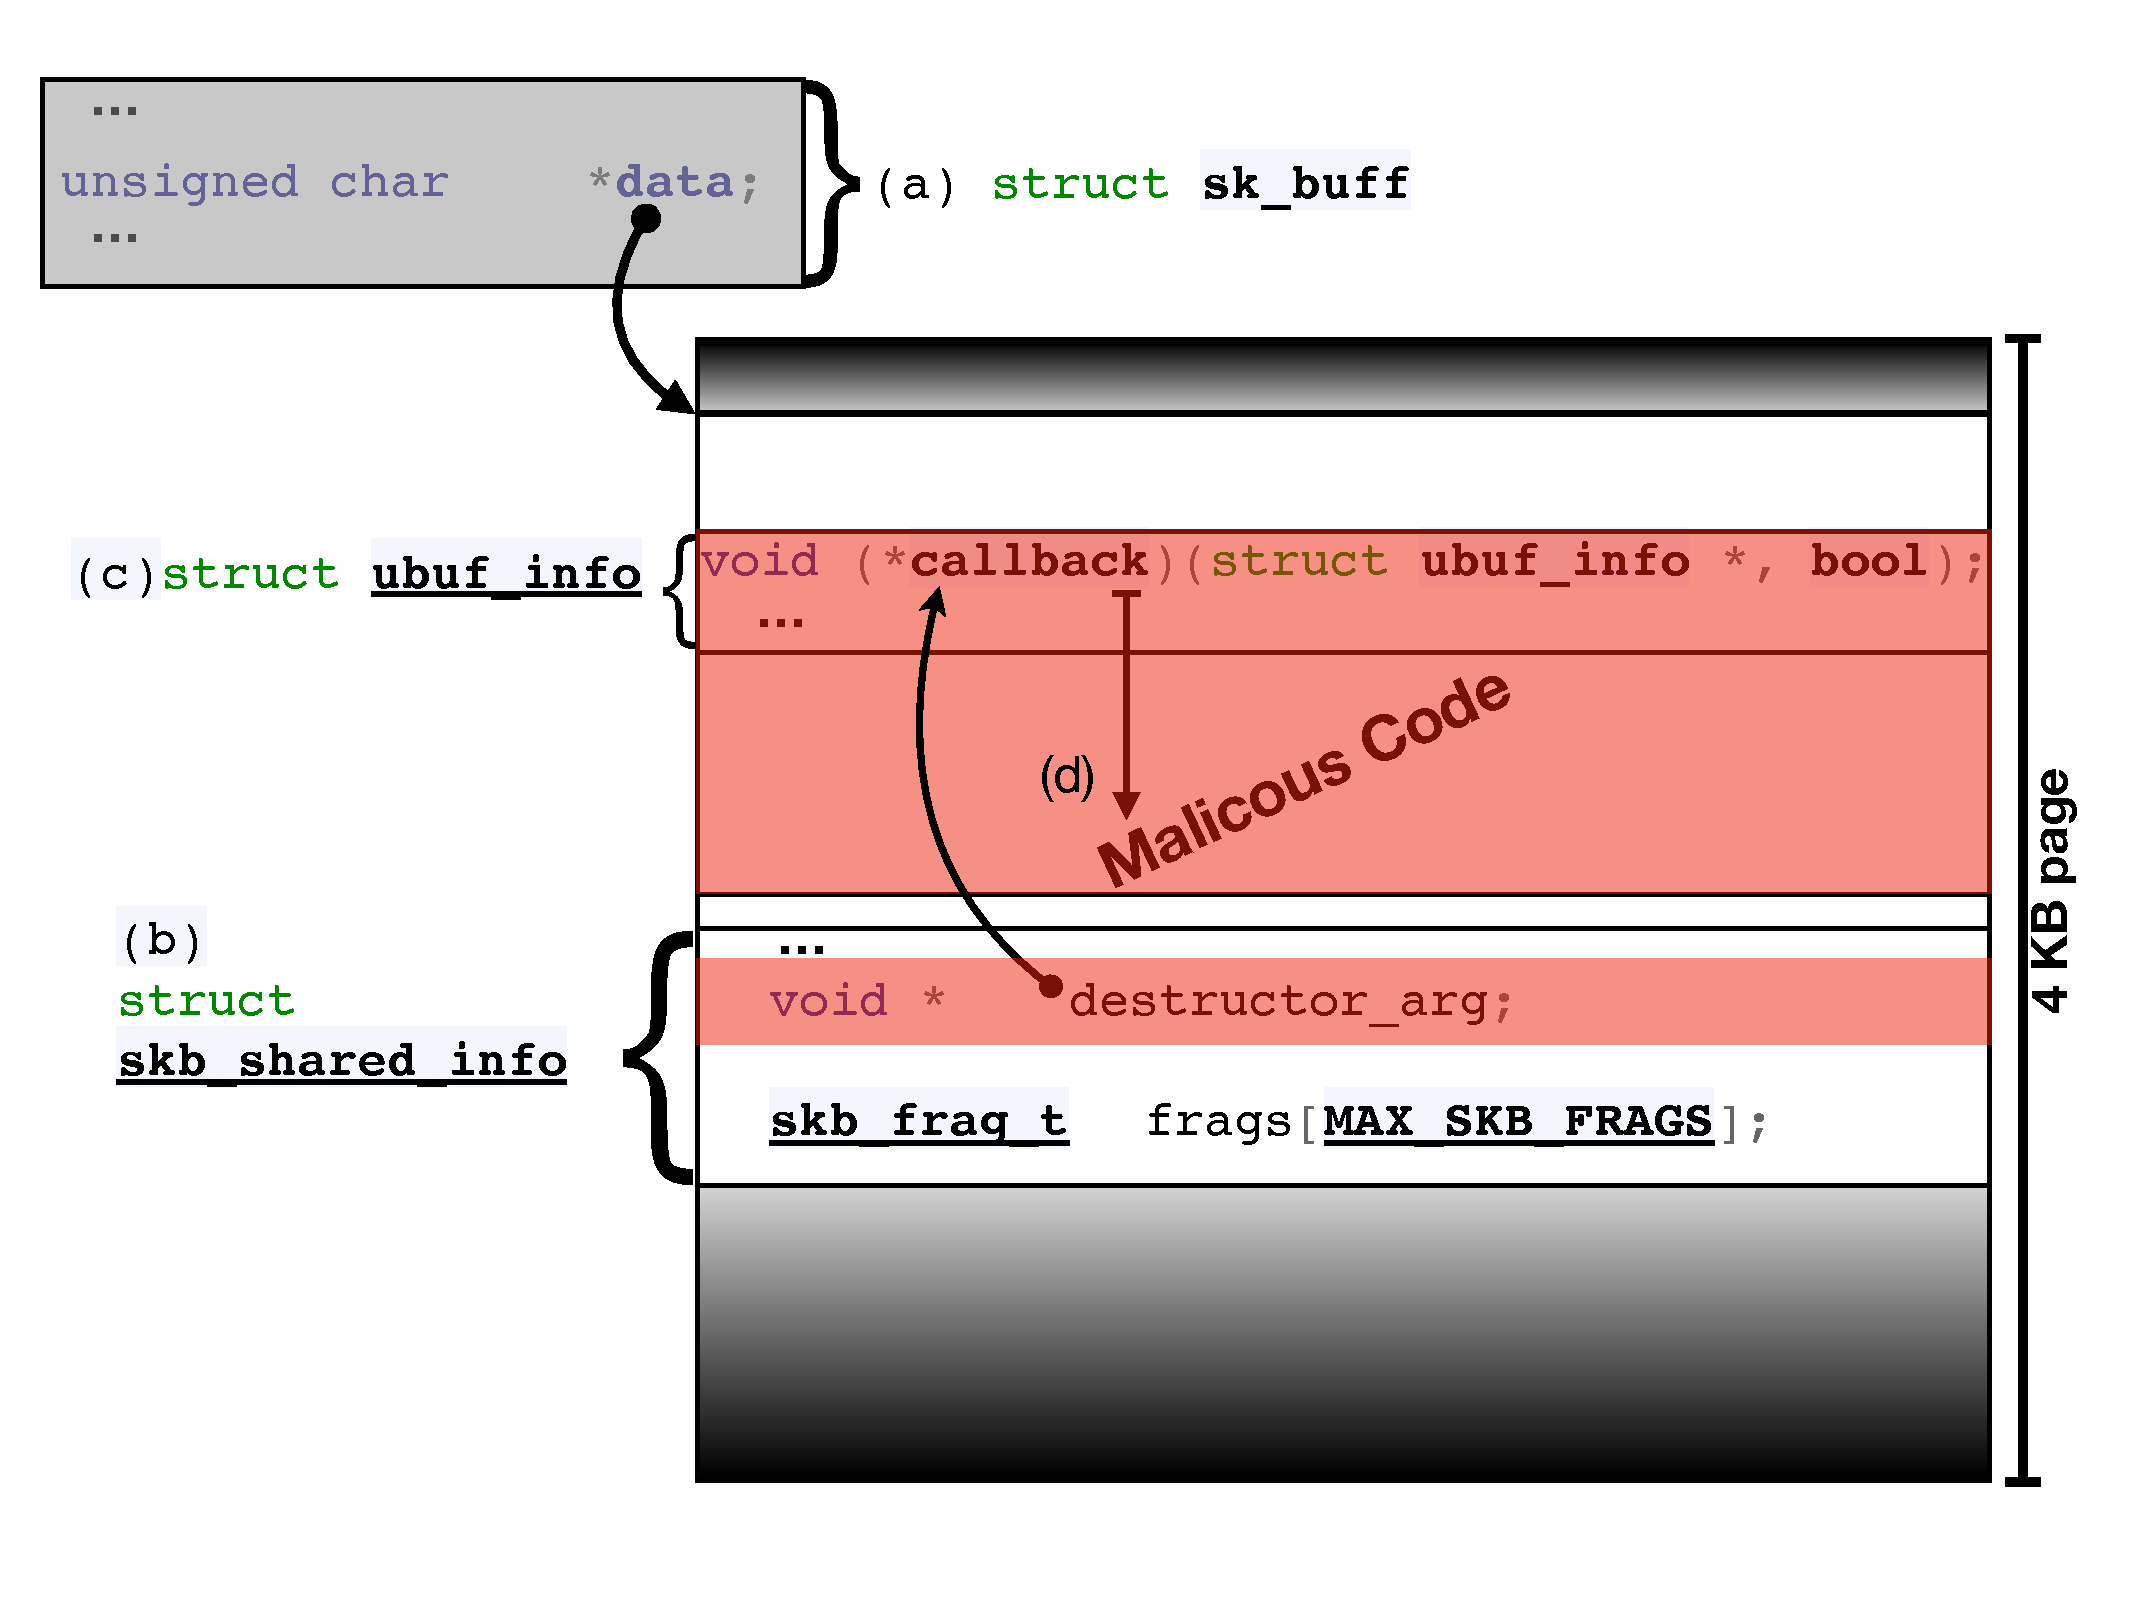
\includegraphics[width=0.8\linewidth]{figs/ubuf.pdf}
    \caption{Using \shinfo{} to execute arbitrary code in \DIFaddbeginFL \DIFaddFL{a }\DIFaddendFL kernel context.}
    \label{fig:sh_info}
    %\vspace{-4mm}
\end{figure}

%\adam{lots of explanations here, whereas the structure was originally mentioned when talking about SCAT...}
Struct \skb{} is a data structure used by the Linux network stack to hold information representing a network packet. Struct \skb{} holds the metadata of a network packet (e.g., packet size, associated socket). One of these fields is a pointer to a data buffer. The data is allocated separately, and thus, does not share a page with its \skb{}\DIFdelbegin \DIFdel{(Fig.~\ref{fig:sh_info})}\DIFdelend \DIFaddbegin \DIFadd{, as shown in Figure~\ref{fig:sh_info}}\DIFaddend . 

This separation means that \skb{} is \emph{never} \DIFdelbegin \DIFdel{(intentionally ) }\DIFdelend \DIFaddbegin \DIFadd{intentionally }\DIFaddend mapped to the device. Indeed, it is a common belief~(e.g., Markettos et al.~\cite{thunder}) \DIFdelbegin \DIFdel{, }\DIFdelend that the Linux network stack is not susceptible to DMA attacks via the \texttt{data} pointer. In this work, we show that this belief is misplaced.

The Linux network stack supports packet cloning by merely copying \skb{} metadata. That is, the resulting \skb{} and the original one share the \texttt{data} buffer~\cite{drivers2005linux}. The payload in the \skb{} can be partially located on the \emph{\DIFdelbegin \DIFdel{liner}\DIFdelend \DIFaddbegin \DIFadd{linear}\DIFaddend } part~(i.e., in the buffer indicated by the \texttt{data} pointer) and partially on the \emph{non-linear} fragments\DIFdelbegin \DIFdel{. That }\DIFdelend \DIFaddbegin \DIFadd{; that }\DIFaddend is, buffers that are described by their \page{}, length\DIFaddbegin \DIFadd{, }\DIFaddend and offset in the \texttt{frags} array of \shinfo{} (\DIFdelbegin \DIFdel{Fig.}\DIFdelend \DIFaddbegin \DIFadd{Figure}\DIFaddend ~\ref{fig:sh_info}). 

To support the sharing of these non-linear buffers, the embedded \shinfo{} metadata structure is used.
Struct \shinfo{}, in contrast to \skb{}, is \emph{always} allocated as part of the data buffer. Therefore it is \emph{always} mapped to the device. \shinfo{} is unwittingly mapped with the permissions of the packet, i.e., WRITE for RX packets, READ for TX packets, and in some cases, such as XDP~\cite{xdp} with BIDIRECTIONAL.

Consequentially, \shinfo{} holds the potential callback pointer that the malicious device can exploit.\footnote{In Fig.~\ref{fig:sh_info} the \texttt{destructor\_arg}\DIFaddbegin \DIFadd{, }\DIFaddend which holds a callback pointer\DIFaddbegin \DIFadd{, }\DIFaddend is used for socket buffer accounting and facilitates custom handling when the buffer is freed.} The \subpage{} vulnerability created by \shinfo{} \DIFdelbegin \DIFdel{, }\DIFdelend represents a type (b) vulnerability (\DIFdelbegin \DIFdel{Fig.}\DIFdelend \DIFaddbegin \DIFadd{Figure}\DIFaddend ~\ref{fig:colocation} (b))\DIFdelbegin \DIFdel{, as }\DIFdelend \DIFaddbegin \DIFadd{: }\DIFaddend this is innate to Linux networking\DIFdelbegin \DIFdel{rather than }\DIFdelend \DIFaddbegin \DIFadd{, as opposed to }\DIFaddend a driver security bug. 

\DIFdelbegin \DIFdel{Fig.}\DIFdelend \DIFaddbegin \DIFadd{Figure}\DIFaddend ~\ref{fig:sh_info} depicts how a malicious device can mount an attack using \shinfo{} in four steps:
\begin{enumerate}[label=(\alph*)]
    \item An RX \skb{} and its data buffer are allocated. The data buffer is mapped for the NIC with WRITE access \DIFdelbegin \DIFdel{(the WRITE access is }\DIFdelend to the whole 4~KB page\DIFdelbegin \DIFdel{)}\DIFdelend . 
    \item The NIC overwrites the \texttt{destructor\_arg} field in \shinfo{} to point within the mapped page. As a result, the \texttt{destructor\_arg} points to a struct \uarg{} \DIFdelbegin \DIFdel{which }\DIFdelend \DIFaddbegin \DIFadd{that }\DIFaddend is created by the NIC.
    \item \uarg{} has a callback pointer that is now pointing to the malicious code residing on the same page. In the case of NX-bit, it is a poisoned ROP/JOP\cite{BJFL11} stack (\DIFdelbegin \DIFdel{Sec.}\DIFdelend \DIFaddbegin \DIFadd{Section}\DIFaddend ~\ref{sec:nx-bit}).
    %\adam{how does this work? you overwrite a pointer to a callback function, not to the stack pointer.}\SV{a JOP attack, aslo mentioned in 2.4}
    \item \DIFdelbegin \DIFdel{when }\DIFdelend \DIFaddbegin \DIFadd{When }\DIFaddend the \skb{} is released, the callback is invoked.
\end{enumerate}
To expand this scenario into a complete attack, the attacker must obtain all three vulnerability attributes. Namely, the attacker needs the actual \kva{} of the \mabaf{} and the NIC must have a timely \DIFaddbegin \DIFadd{window for }\DIFaddend WRITE access to the page. Next, we demonstrate how an attacker can leverage standard OS behavior to obtain both missing \mbox{vulnerability attributes.}

\begin{figure}[t]
    \centering
    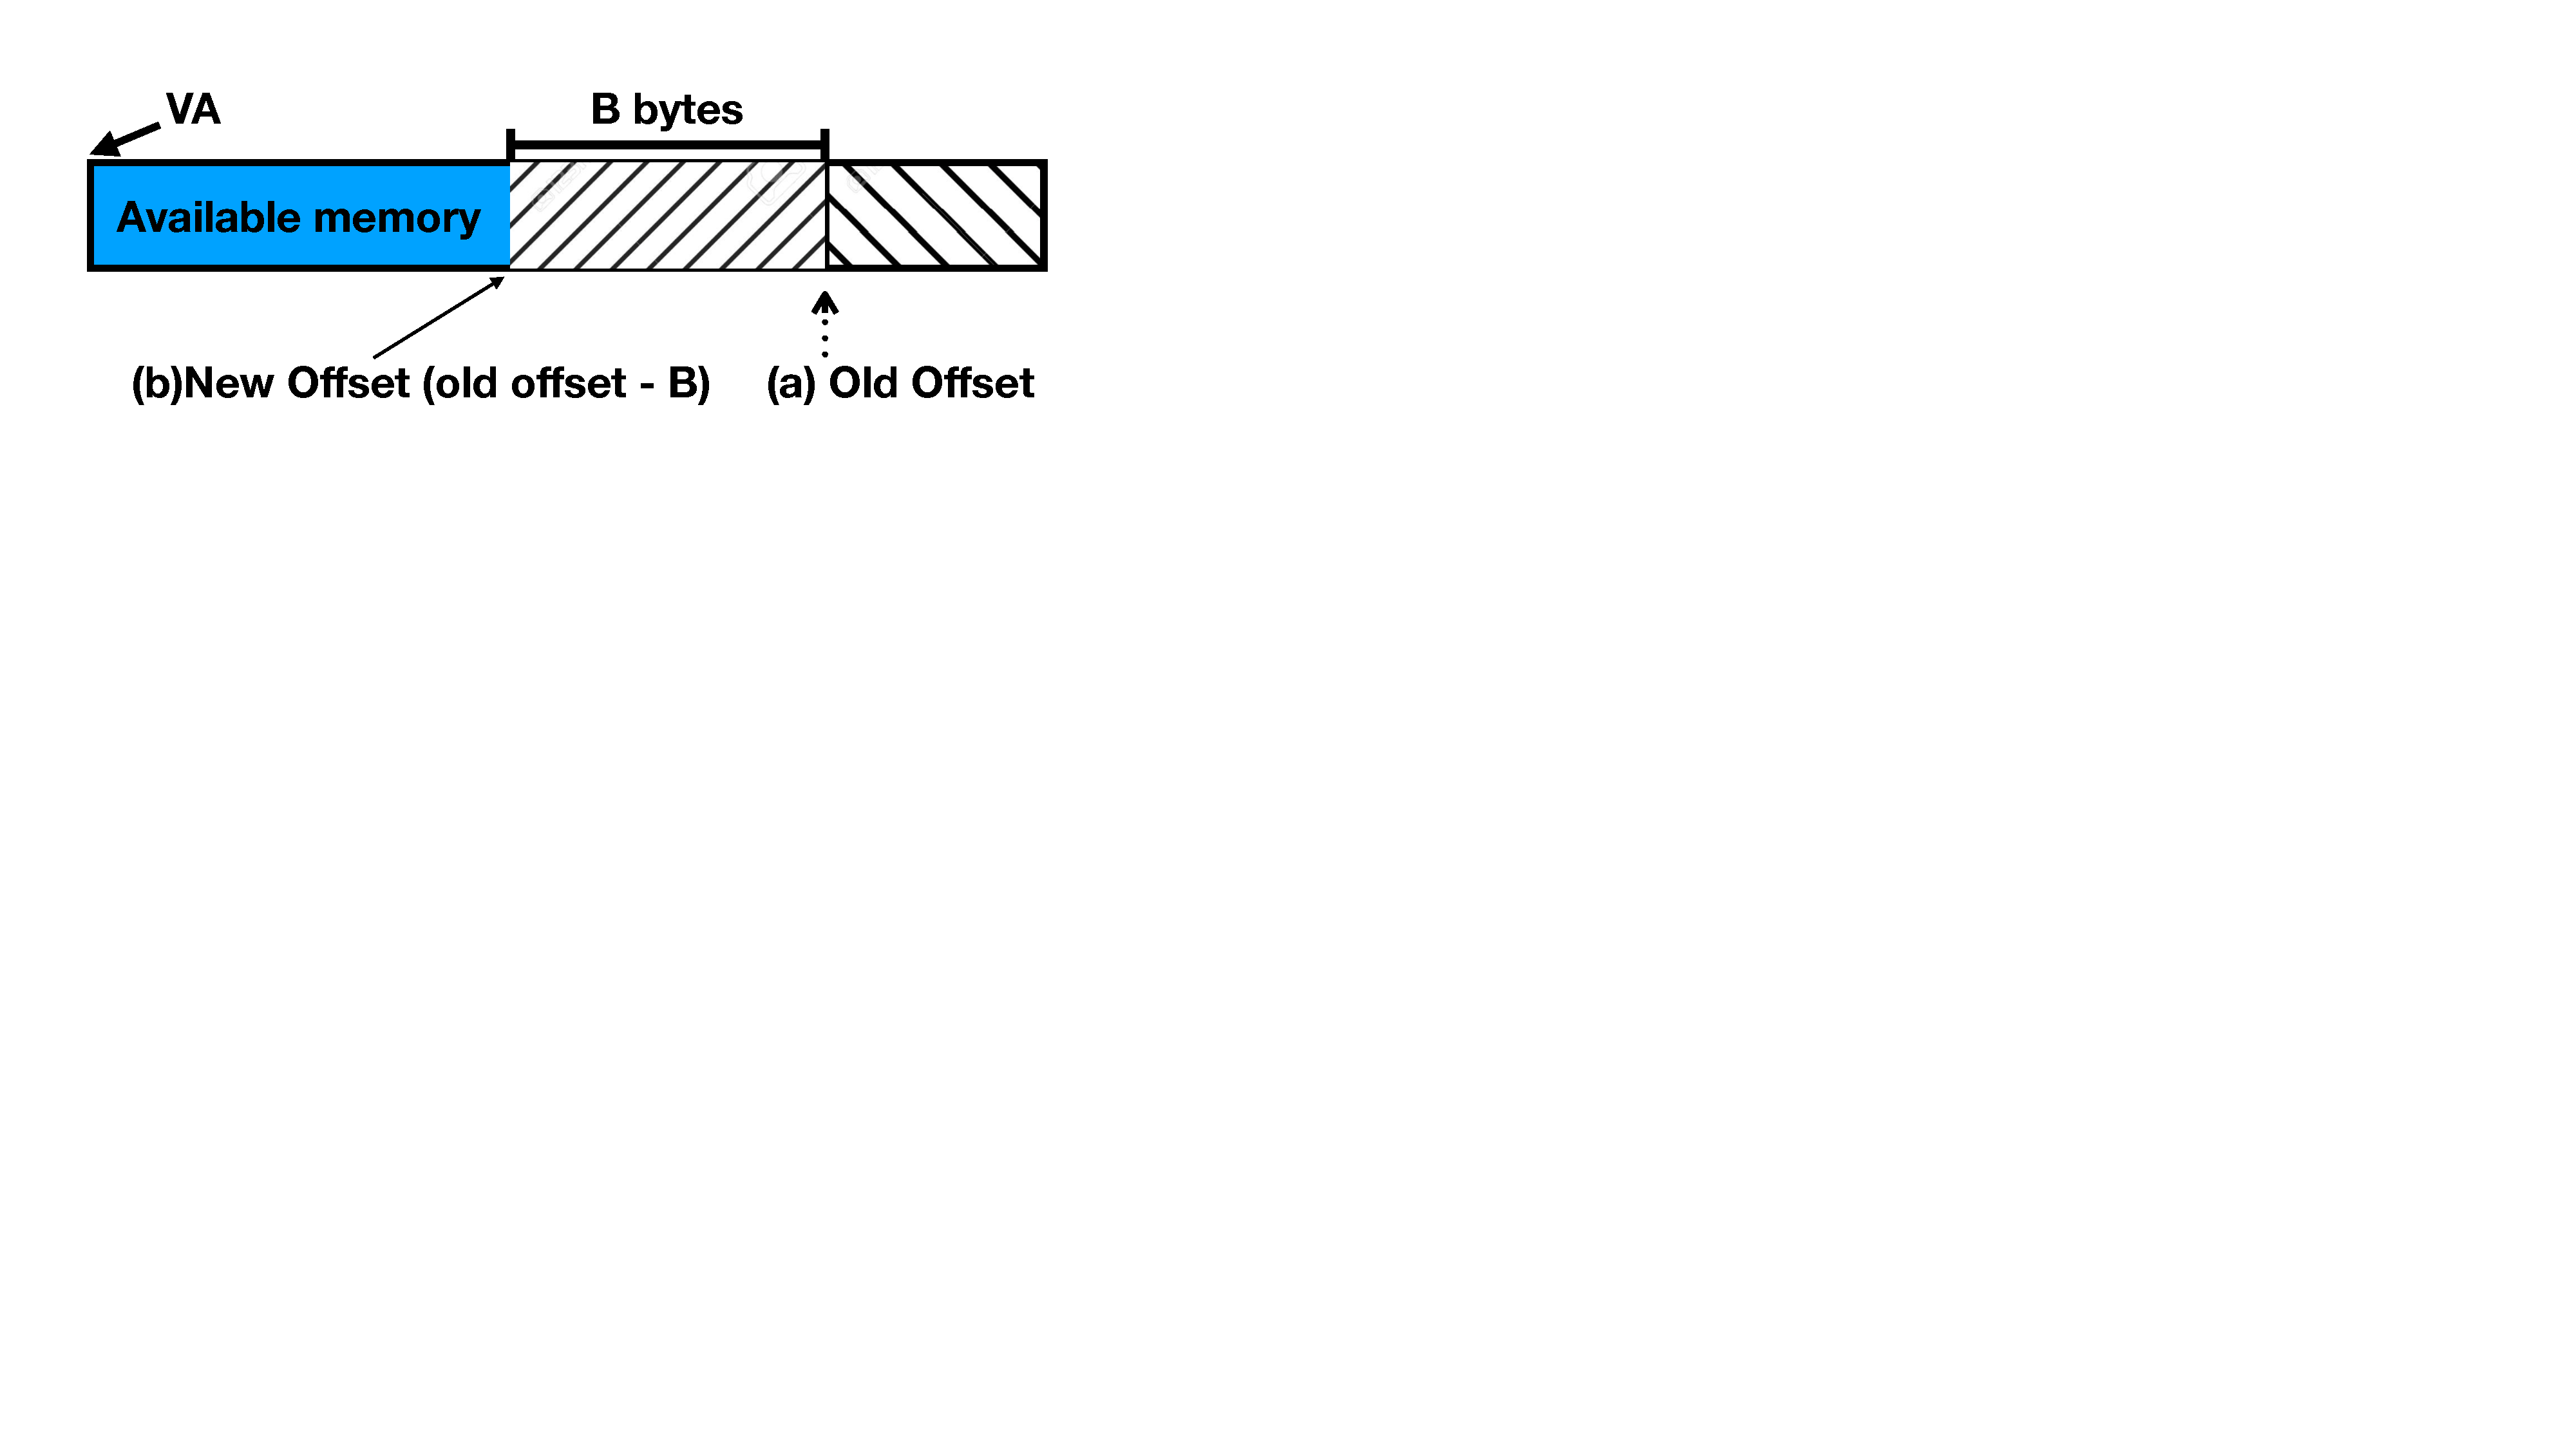
\includegraphics[width=0.65\linewidth,trim=0 6cm 0 6cm, clip]{figs/page_frag.pdf}
    \caption{Allocation of B bytes from page\_frag}
    \label{fig:page_frags}
\end{figure}

\subsection{Existence of a Time Window}\label{sec:timely}
To reason about the existence of an appropriate time window for altering the callback pointer, we first discuss the Linux default mode for IOTLB invalidation, which is a known security vulnerability~\cite{MMT16,MSMT18}.
In \DIFdelbegin \DIFdel{particular, in Sec.~\ref{sec:deferred}}\DIFdelend \DIFaddbegin \DIFadd{Section~\ref{sec:deferred}, }\DIFaddend we present the issue of deferred invalidation. Then, in \DIFdelbegin \DIFdel{Sec.~\ref{sec:shinfo}}\DIFdelend \DIFaddbegin \DIFadd{Section~\ref{sec:shinfo}, }\DIFaddend we discuss the multiple means by which an attacker can gain timely access to \shinfo.

\subsubsection{Deferred Invalidation Vulnerability}\label{sec:deferred}
The IOTLB is analogous to the MMU TLB. The IOMMU does not maintain consistency between the IOTLB and the IOMMU page tables. As a result, the OS has to explicitly invalidate the IOTLB to maintain consistency when a translation entry is removed. \DIFdelbegin \DIFdel{Namely, to }\DIFdelend \DIFaddbegin \DIFadd{To }\DIFaddend ensure that the IOTLB never holds stale entries, the OS must invalidate the IOTLB entry immediately after removing a DMA mapping. 

This scheme, called \emph{strict} mode in Linux, can degrade performance due to the overhead of IOTLB invalidations following each I/O operation ~\cite{MMT16,MSMT18,Peleg15}. In I/O intensive workloads, the combined cost of IOTLB invalidations can be prohibitively high. The overhead of each IOTLB invalidation can be as high as 2000 cycles~\cite{ABYTS11}. This overhead is considerably higher than a TLB invalidation, which takes roughly 100 cycles~\cite{Han14}. 

To reduce this overhead, Linux uses deferred mode as a default. Linux defers specific IOTLB invalidations and instead performs periodic global IOTLB invalidations. While this \emph{deferred} mode improves I/O performance, it also breaks the stipulation that after unmapping (e.g., \texttt{dma\_unmap\_page}), the physical page should no longer be accessible by the device. This \emph{deferred} time frame\DIFdelbegin \DIFdel{(Fig.}\DIFdelend \DIFaddbegin \DIFadd{, shown in Figure}\DIFaddend ~\ref{fig:deferred})\DIFaddbegin \DIFadd{, }\DIFaddend may be as high as 10 milliseconds~\cite{MSMT18}.

The repercussions of \emph{deferred} mode are that a malicious device can take advantage of this time window, where it has access to memory pages unbeknownst to the CPU. \DIFaddbegin \DIFadd{The }\DIFaddend \emph{deferred} mode opens up two distinct attack options:

\begin{enumerate}[labelindent=0pt]
    \item A device can alter data structures that the CPU has modified \emph{after} unmapping (e.g., calling \texttt{dma\_unmap\_page}).
    \iova{} mappings, as a rule, are short-lived as they \DIFdelbegin \DIFdel{should }\DIFdelend \DIFaddbegin \DIFadd{are meant }\DIFaddend be used only for the duration of \DIFaddbegin \DIFadd{the }\DIFaddend I/O, usually for a few microseconds. The additional milliseconds provide the attacker with a \DIFdelbegin \DIFdel{wide time window sufficient }\DIFdelend \DIFaddbegin \DIFadd{time window wide enough }\DIFaddend to conduct its attack.
    \item The page can be freed and then immediately reused by the OS. Fast reuse is a common scenario since Linux reuses \emph{hot} pages (i.e., recently used pages) as they are likely to reside in the CPU caches~\cite{hotcold}. However, this also \DIFdelbegin \DIFdel{opens up the kernel }\DIFdelend \DIFaddbegin \DIFadd{leaves the kernel open }\DIFaddend to additional random exposure attacks.
\end{enumerate}



\begin{figure}[t]
    \centering
    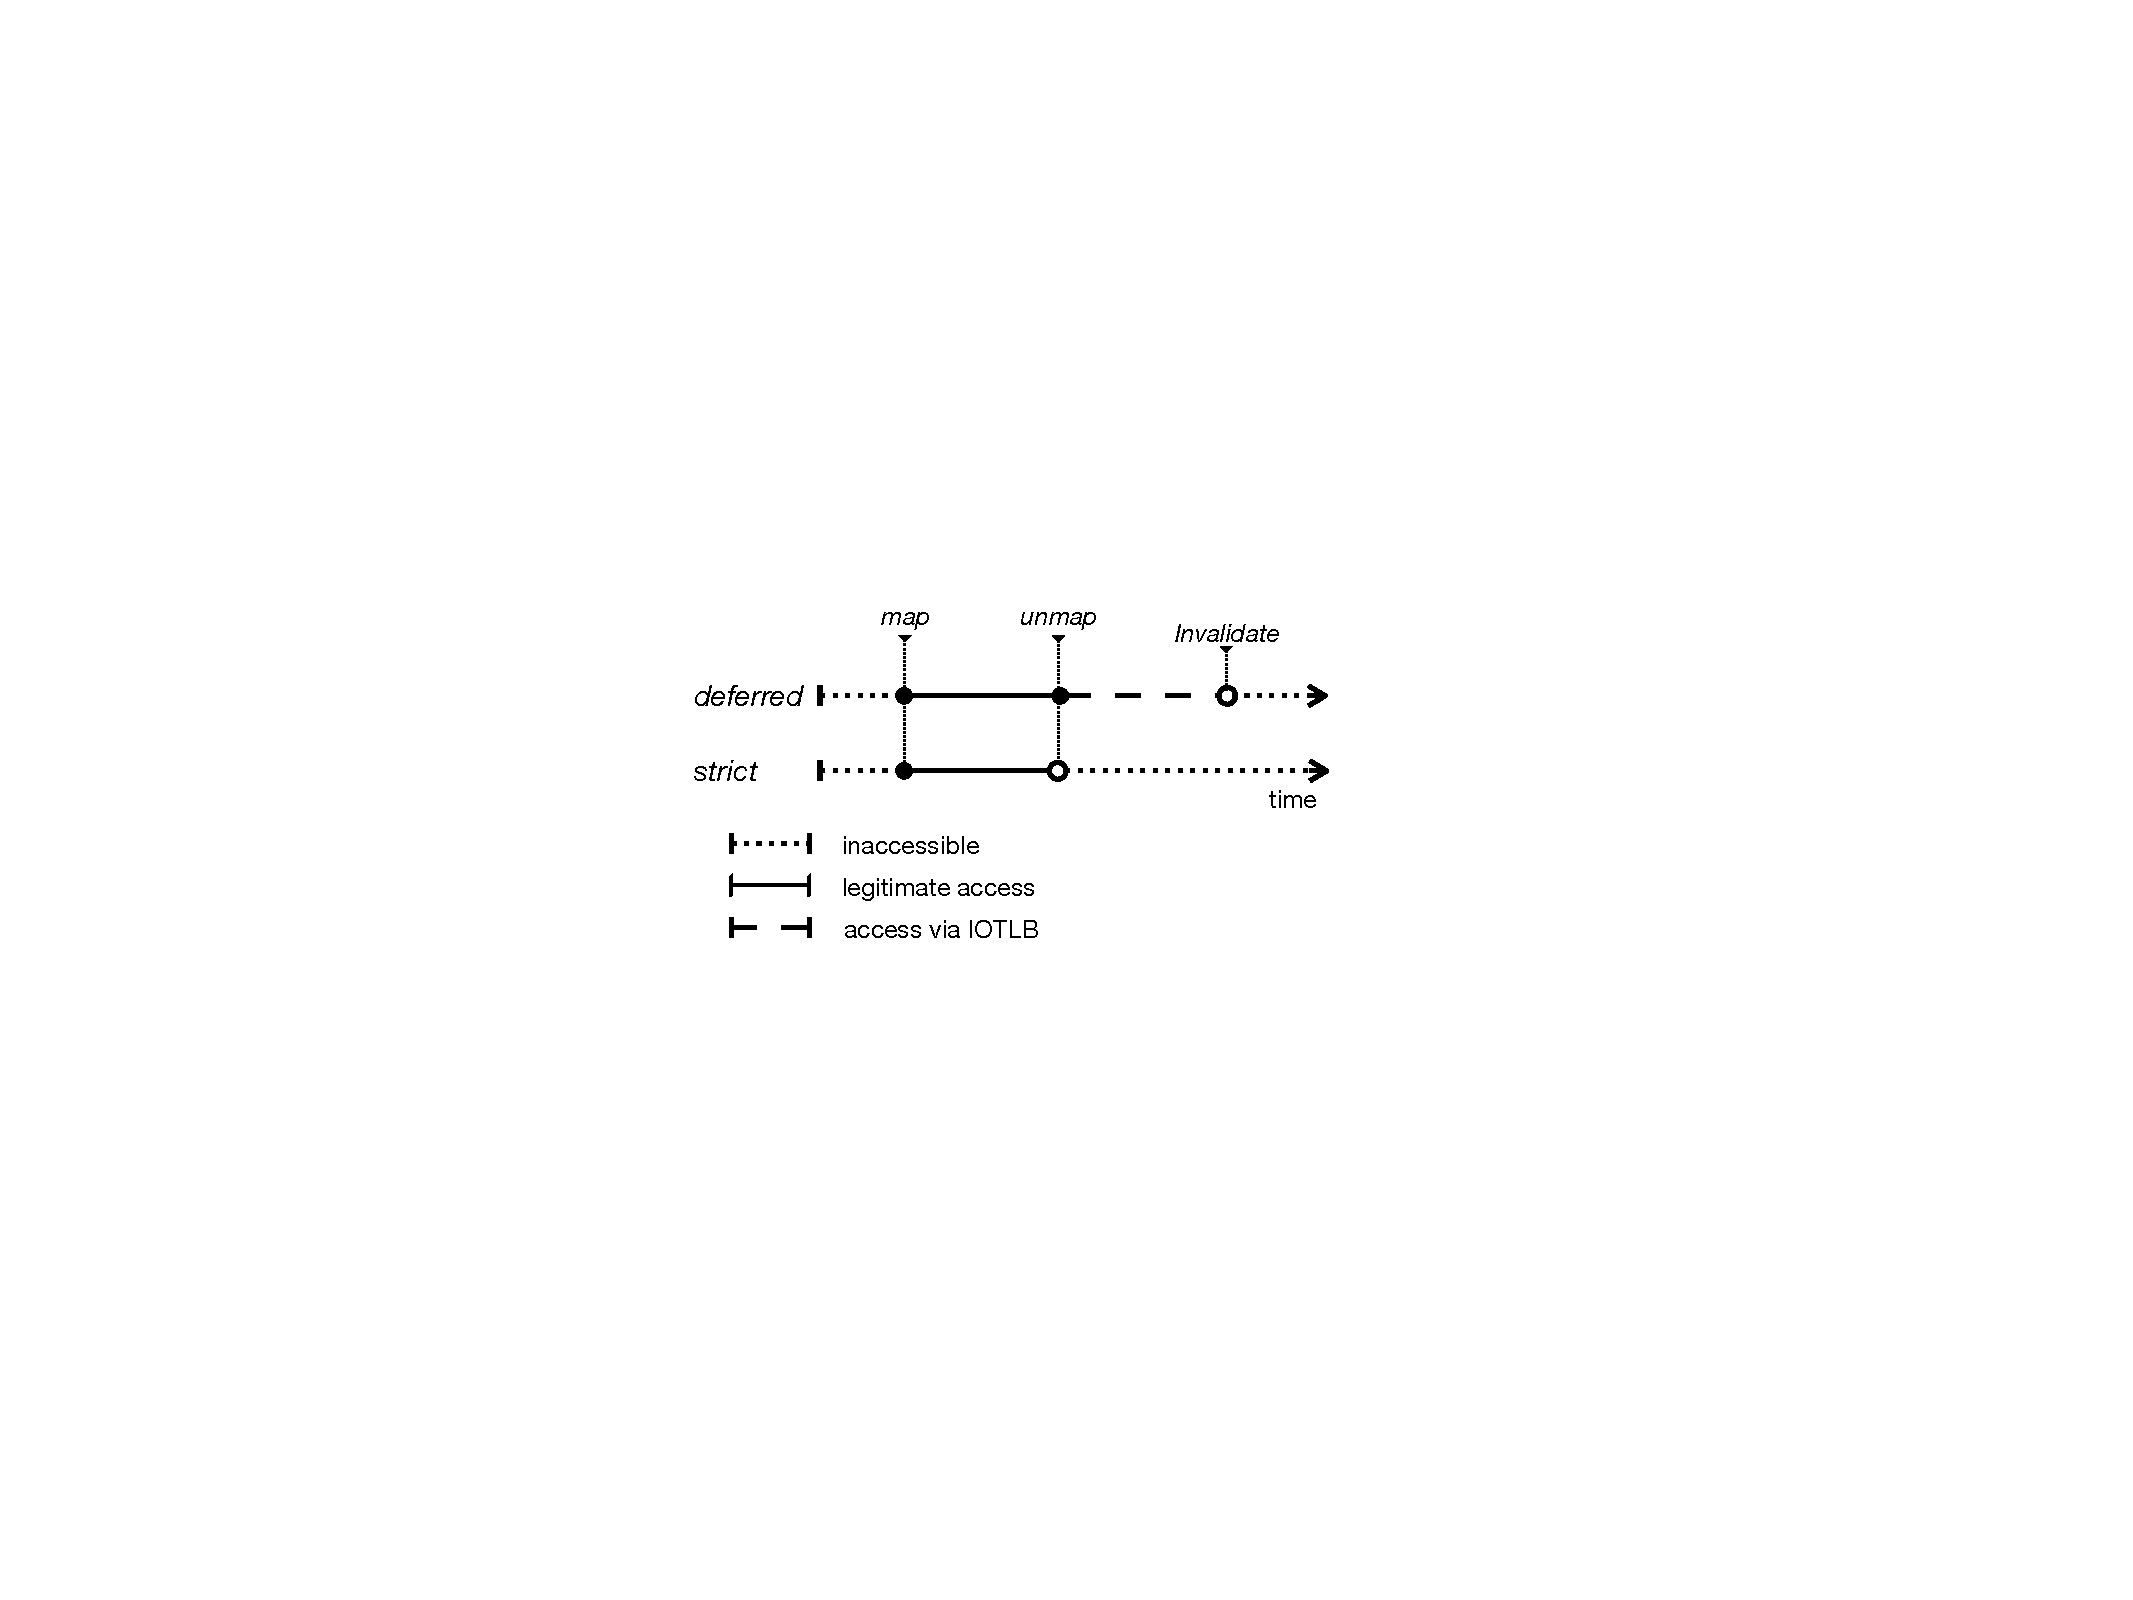
\includegraphics[width=0.75\columnwidth]{figs/strict.pdf}
    \caption{Strict vs. deferred IOTLB invalidation. In \emph{deferred} mode, there is a time window \DIFdelbeginFL \DIFdelFL{where }\DIFdelendFL \DIFaddbeginFL \DIFaddFL{in which }\DIFaddendFL the data is accessible to the device, but the mapping no longer appears in the page table.}
    \label{fig:deferred}
\end{figure}

\subsubsection{\DIFdelbegin \DIFdel{The }\DIFdelend Time \DIFdelbegin \DIFdel{window}\DIFdelend \DIFaddbegin \DIFadd{Window}\DIFaddend }\label{sec:shinfo}

\begin{figure}[t]
    \centering
    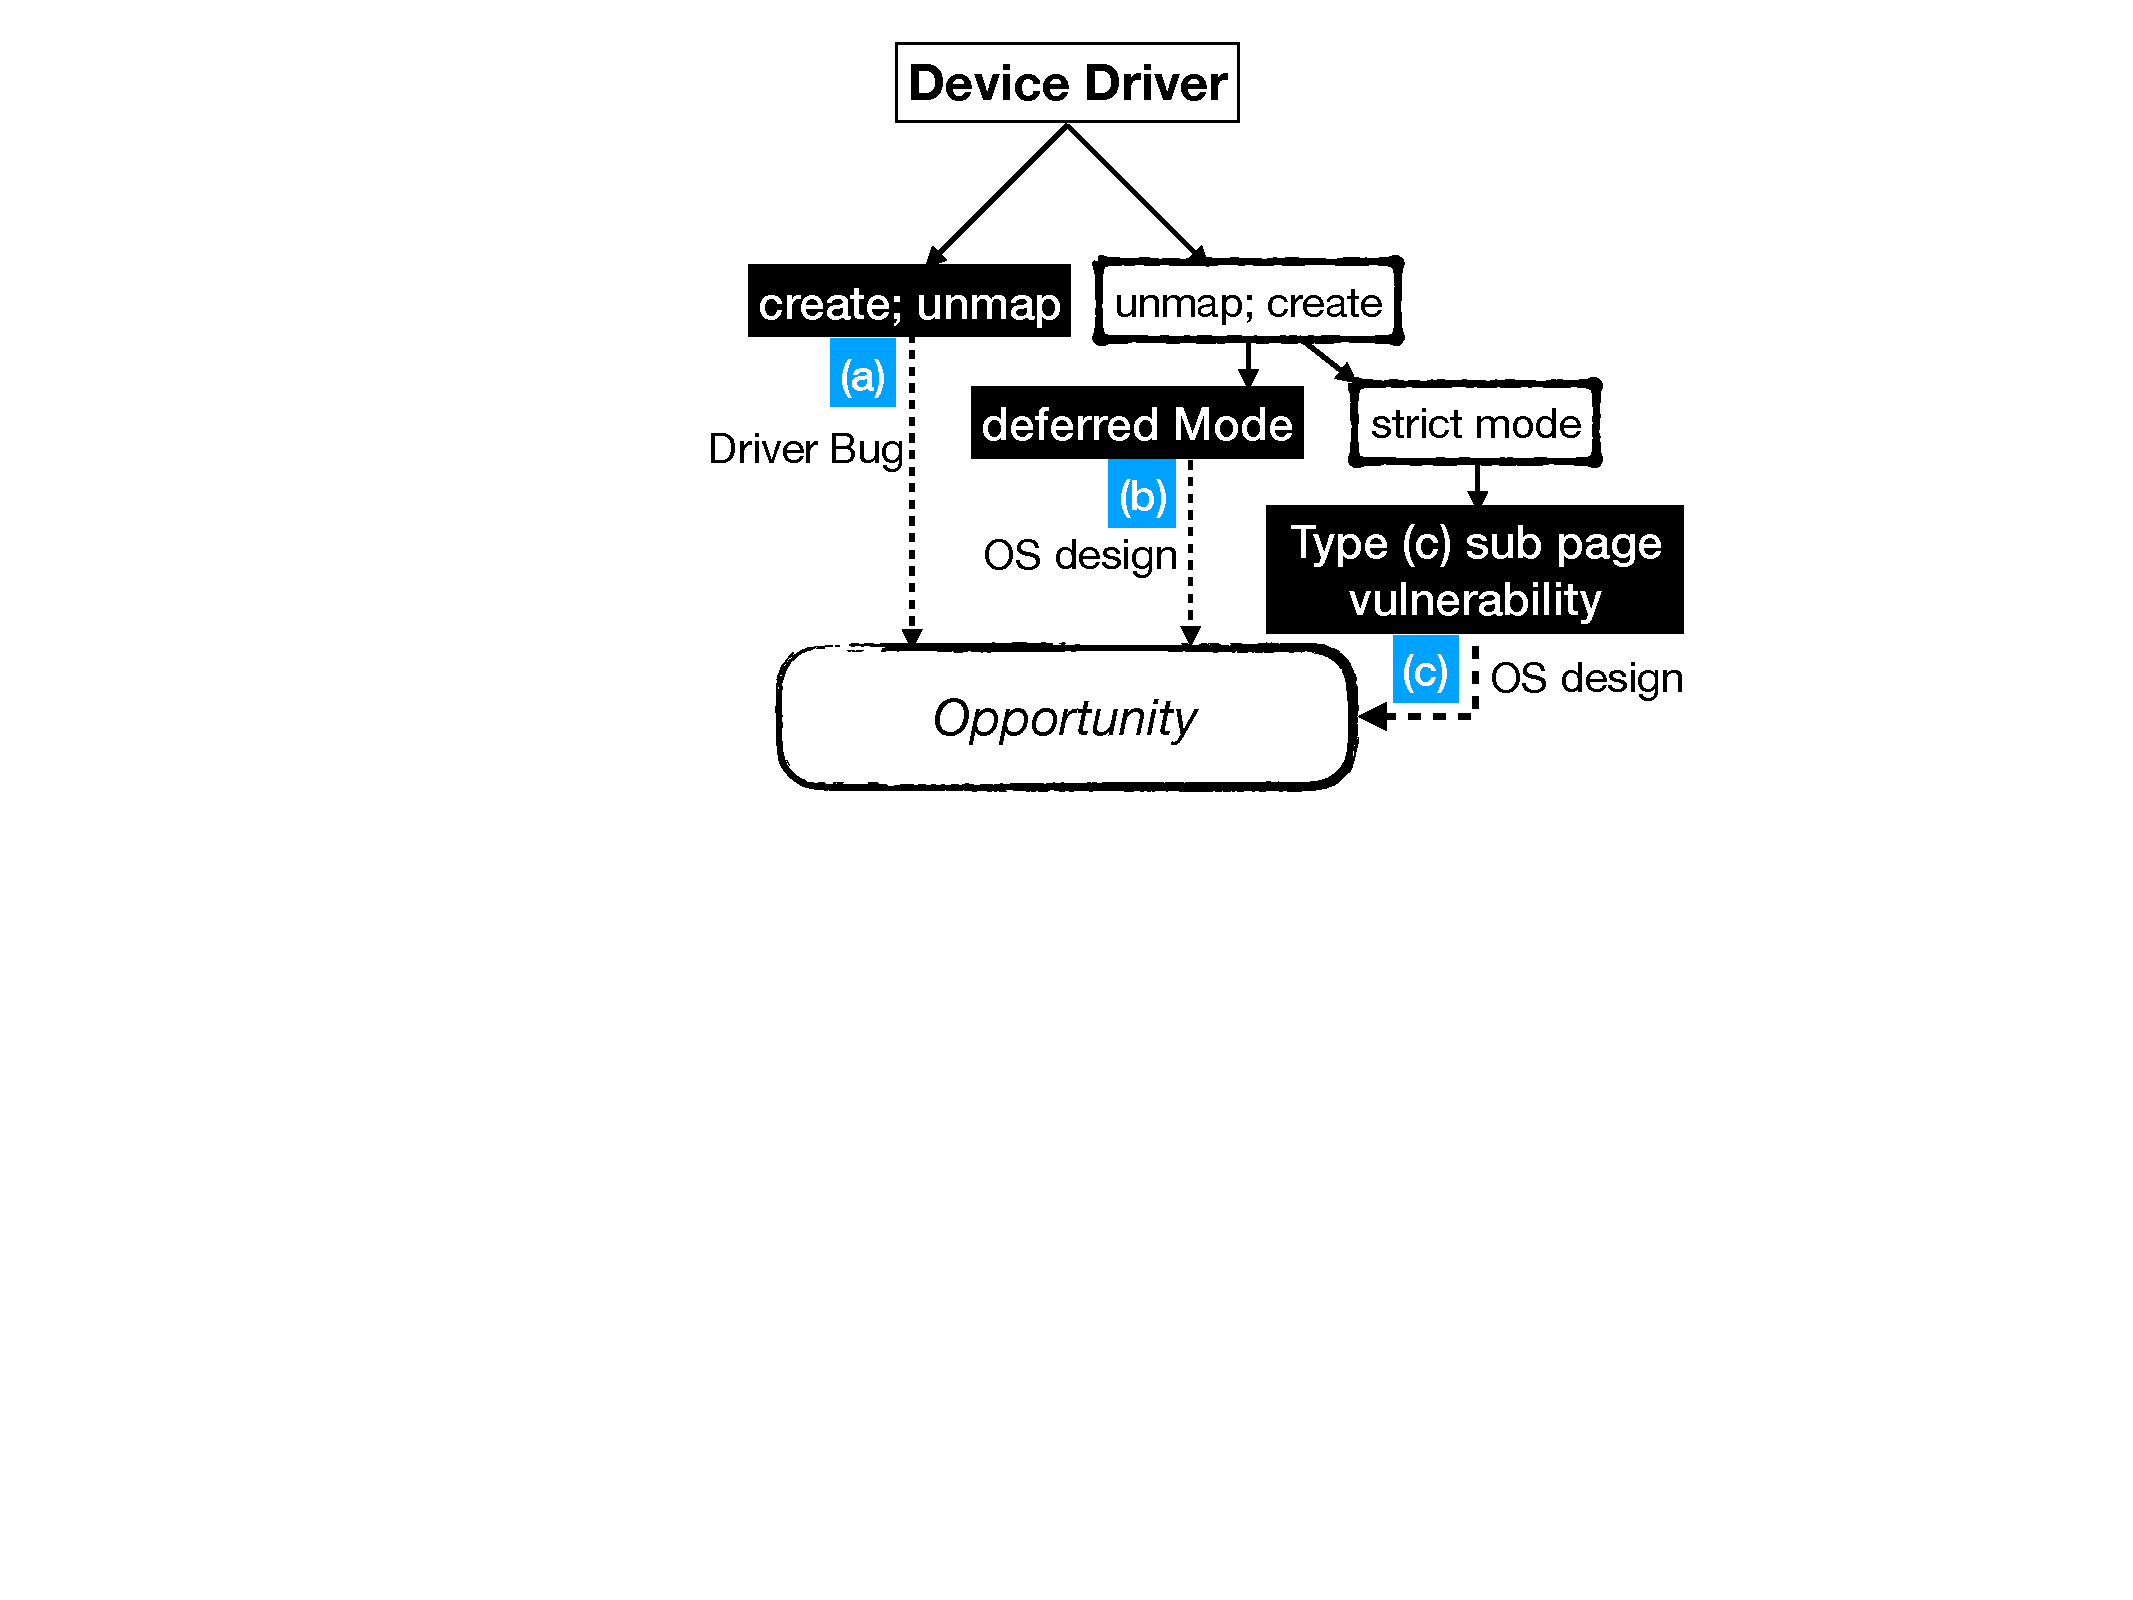
\includegraphics[width=0.75\linewidth]{figs/road_to_op.pdf}
    \caption{Different ways in which the callback pointer in \shinfo can be successfully exploited.}
    %\vspace{-2mm}
    \label{fig:road_to_op}
\end{figure}

%\adam{IMPORTANT POINT: To me, it seemed that the tool sections were about gaining Opportunity.  Why do we now need another section on "Hacking" it? Do the tools not flag the skb-shared-info? If they do, and it's still not enough, how do we know Opportunity exists in the other cases they flag?  Perhaps, the exact goal of the tools and what they find should be described more precisely.}
%\st{We now detail the different ways in which a malicious device can obtain} \oportunity{} (Fig.~\ref{fig:road_to_op}).

%In this section we discuss the Linux network stack where \shinfo is initialized \emph{after} the page was unmapped, thus invalidating the malicious changes.
\DIFdelbegin \DIFdel{Upon packet arrival }\DIFdelend \DIFaddbegin \DIFadd{When a packet arrives }\DIFaddend on a receive path, an \shinfo struct is \DIFdelbegin \DIFdel{initialised after a }\DIFdelend \DIFaddbegin \DIFadd{initialized after the }\DIFaddend packet is received \DIFdelbegin \DIFdel{, namely }\DIFdelend \DIFaddbegin \DIFadd{i.e., }\DIFaddend after the DMA operation was completed and \DIFdelbegin \DIFdel{potentially }\DIFdelend the DMA access \DIFaddbegin \DIFadd{is potentially }\DIFaddend revoked. In such a case,
\DIFdelbegin \DIFdel{a }\DIFdelend correct use of the DMA API should thwart the attack outlined in \DIFdelbegin \DIFdel{Sec.}\DIFdelend \DIFaddbegin \DIFadd{Section}\DIFaddend ~\ref{sec:shinfo_exploit} (\DIFdelbegin \DIFdel{Fig.}\DIFdelend \DIFaddbegin \DIFadd{Figure}\DIFaddend ~\ref{fig:sh_info}). \DIFdelbegin \DIFdel{Namely, first }\DIFdelend \DIFaddbegin \DIFadd{First }\DIFaddend unmapping the buffer and only then initializing the \shinfo{} should allow the CPU to undo any malicious changes \DIFaddbegin \DIFadd{made }\DIFaddend by the NIC. But, as we next demonstrate, DMA access is often easily \DIFdelbegin \DIFdel{achievable }\DIFdelend \DIFaddbegin \DIFadd{achieved }\DIFaddend even after the CPU has made its changes. 

We \DIFdelbegin \DIFdel{next }\DIFdelend \DIFaddbegin \DIFadd{now }\DIFaddend describe how the time window is attainable via three different paths\DIFaddbegin \DIFadd{, }\DIFaddend as illustrated in \DIFdelbegin \DIFdel{Fig.}\DIFdelend \DIFaddbegin \DIFadd{Figure}\DIFaddend ~\ref{fig:road_to_op}: 

%\adam{why is this an enumerations?}\SV{added reference to figure 8...}

\begin{enumerate}[label=(\roman*),wide, labelwidth=!, labelindent=0pt]

\item \DIFdelbegin \DIFdel{As it turns out}\DIFdelend \DIFaddbegin \DIFadd{Apparently}\DIFaddend , prevalent device drivers (e.g., Intel 40GbE driver, i40e) first create an \skb{} and only then unmap the buffer. This order of execution allows the \emph{device} to undo legitimate changes to \shinfo{} by the CPU. 

\item \DIFdelbegin \DIFdel{Nevertheless, even }\DIFdelend \DIFaddbegin \DIFadd{Even }\DIFaddend when the order is correct \DIFdelbegin \DIFdel{, i.e., }\DIFdelend \DIFaddbegin \DIFadd{and }\DIFaddend the unmapping of the buffer occurs before the creation of the \skb{},  \DIFdelbegin \DIFdel{still }\DIFdelend \shinfo{} is \DIFdelbegin \DIFdel{not safe }\DIFdelend \DIFaddbegin \DIFadd{still not secure }\DIFaddend from later modifications. \DIFdelbegin \DIFdel{As }\DIFdelend \DIFaddbegin \DIFadd{Because }\DIFaddend the default IOMMU mode in Linux is \emph{deferred} protection (\DIFdelbegin \DIFdel{Sec.}\DIFdelend \DIFaddbegin \DIFadd{Section}\DIFaddend ~\ref{sec:deferred}), the unmap order is made irrelevant. \DIFdelbegin \DIFdel{That is, even }\DIFdelend \DIFaddbegin \DIFadd{Even }\DIFaddend though the unmap function is invoked in the correct order, the device can still corrupt \shinfo{} due to the IOTLB.  

\item In response, a security-conscious admin may change the default setting to \emph{strict} mode, where the IOTLB is flushed \DIFdelbegin \DIFdel{on }\DIFdelend \DIFaddbegin \DIFadd{at }\DIFaddend every unmap. However, this \DIFdelbegin \DIFdel{both }\DIFdelend severely degrades networking performance~\cite{MMT16,MSMT18} \DIFdelbegin \DIFdel{, }\DIFdelend and does not alleviate the security threats on the system. Presumably, with \emph{strict} mode enabled, the \iova{} \DIFdelbegin \DIFdel{the NIC used }\DIFdelend \DIFaddbegin \DIFadd{that is used by the NIC }\DIFaddend to access that \shinfo{} is no longer valid\DIFdelbegin \DIFdel{, which }\DIFdelend \DIFaddbegin \DIFadd{. This }\DIFaddend initially sounds promising. The problem is that \DIFdelbegin \DIFdel{the device, }\DIFdelend in many cases \DIFdelbegin \DIFdel{, }\DIFdelend \DIFaddbegin \DIFadd{the device }\DIFaddend still has legitimate WRITE access to the physical page of the \shinfo. The vulnerability stems from the way \data{} is allocated. An RX \skb{} is almost exclusively allocated via an API (e.g., \texttt{netdev\_alloc\_skb}) that creates a type (c) \subpage{} vulnerability (\DIFdelbegin \DIFdel{Fig.}\DIFdelend \DIFaddbegin \DIFadd{Figure}\DIFaddend ~\ref{fig:colocation}(c)). The device can use the \iova{} of a co-located buffer to access the \shinfo{} it requires. \DIFdelbegin \DIFdel{Particularly}\DIFdelend \DIFaddbegin \DIFadd{Specifically}\DIFaddend , the buffers of the driver RX ring are allocated sequentially, resulting in pairs of successive RX descriptors that map the same page. Obviously, this holds as long as the buffer sizes are smaller than 4 KB. This is a reasonable assumption since the default MTU size is 1500~B. These allocation functions, use a \texttt{page\_frag} mechanism to allocate the \data{} buffers, which in turn contain \shinfo. The \texttt{page\_frag} is an efficient method for allocating small buffers, \DIFaddbegin \DIFadd{and is }\DIFaddend often used by the Linux network stack\DIFdelbegin \DIFdel{(}\DIFdelend \DIFaddbegin \DIFadd{. In fact, }\DIFaddend it is used 344 times by network drivers in Linux kernel 5.0\DIFdelbegin \DIFdel{)}\DIFdelend . A \texttt{page\_frag} is initialized by allocating a contiguous memory region (usually 32 KB), setting a \textit{va} pointer to the beginning of the region\DIFdelbegin \DIFdel{and }\DIFdelend \DIFaddbegin \DIFadd{, and setting an }\DIFaddend \texttt{offset} to the end. An allocation request for \texttt{B} bytes subtracts \texttt{B} bytes from the \texttt{offset} pointer and returns the new value of \DIFaddbegin \DIFadd{the }\DIFaddend \texttt{offset}. In multi-core environments, the \texttt{page\_frag} uses a different buffer for each CPU and each CPU has a single RX ring. As a result, each RX ring is served by its own (per-CPU) contiguous buffer\DIFdelbegin \DIFdel{. (Fig.}\DIFdelend \DIFaddbegin \DIFadd{, as show in Figure}\DIFaddend ~\ref{fig:page_frags}). This mechanism for memory allocation results in consecutive \data{} buffers often residing on the same memory page. Due to this type (c) \subpage{} vulnerability, the NIC does not require the invalidated \iova{} to modify the \shinfo. Instead, it can use the \iova{} for the next data buffer.\footnote{Note that the lower 12 bits (\DIFaddbegin \DIFadd{i.e., }\DIFaddend the offset on the page) of the \iova{} are identical to the corresponding \kva{} bits.} The device still has write access due to the valid \iova of the next buffer (i.e., the striped area at the end of the page \DIFdelbegin \DIFdel{at Fig.}\DIFdelend \DIFaddbegin \DIFadd{in Figure}\DIFaddend ~\ref{fig:sh_info}).
\end{enumerate}

% \smallskip
% \noindent\textbf{\sout{Our setup.}} \sout{The tg3 and mlx5\_core are both vulnerable. The tg3 driver uses the correct unmapping order, but uses the \texttt{netdev\_alloc\_frag} function that results in a type (c) \subpage{} vulnerability. mlx5\_core driver avoids unmapping the RX buffers altogether. \sout{In kernel 5.0, the driver uses a \texttt{page\_pool} mechanism~\cite{page_pool}.} These design choices leave \shinfo{} vulnerable, in both cases, regardless of the IOMMU policy (i.e., \emph{deferred} or \emph{strict}).}


From this point on, we assume that the attacker can always modify the callback pointer. In the next subsections, we demonstrate various compound DMA attacks \DIFdelbegin \DIFdel{where }\DIFdelend \DIFaddbegin \DIFadd{in which }\DIFaddend an attacker can exploit the OS design to obtain the kernel virtual address of buffers containing malicious code\DIFdelbegin \DIFdel{, completing }\DIFdelend \DIFaddbegin \DIFadd{; this completes }\DIFaddend the trifecta of vulnerabilities.

\subsection{\DIFdelbegin \DIFdel{The Ring Flood }\DIFdelend \DIFaddbegin \DIFadd{RingFlood }\DIFaddend \Compound{} Attack}\label{sec:ringflod}
A malicious device can generate a poisoned ROP stack in each RX buffer.
However, this is not sufficient to execute a successful code injection attack \DIFdelbegin \DIFdel{. 
In particular, }\DIFdelend \DIFaddbegin \DIFadd{since }\DIFaddend the device has all the \iova{} for the RX buffers, but not the \kva{}.
%since the device lacks the corresponding \kva of the RX buffer.

%A malicious device can generate a poisoned ROP stack in each RX buffer. At this point, the device still cannot execute a successful code injection attack since it lacks the corresponding \kva of the RX buffer.
%The device has all the \iova{} for the RX buffers, but not the \kva{}. 

In this attack, we take advantage of the fact that the boot process is \emph{deterministic}. \DIFdelbegin \DIFdel{Each }\DIFdelend \DIFaddbegin \DIFadd{At every }\DIFaddend reboot, the same set of commands is executed in the same order, initiating the same kernel modules and starting the same processes. While the pages each module receives may vary in a multi-core environment due to timing issues, we do not expect the drift to be too large. 

We \DIFdelbegin \DIFdel{evaluate }\DIFdelend \DIFaddbegin \DIFadd{evaluated }\DIFaddend this assumption on our setup\DIFaddbegin \DIFadd{, }\DIFaddend running 256 reboots on Ubuntu 18.04 with \DIFdelbegin \DIFdel{both }\DIFdelend \DIFaddbegin \DIFadd{Linux }\DIFaddend kernels 5.0 and 4.15. With the mlx5\_core driver, many PFNs repeat in more than 50\%  \DIFdelbegin \DIFdel{percent }\DIFdelend of reboots on kernel 5.0 and more than 95\% on kernel 4.15. The 4.15 driver version allocates much more memory, allocating 64~KB per RX buffer to facilitate the HW LRO feature. We assume an attacker can gain access to an identical setup and identify the most common PFN. Therefore, an adversary with knowledge about the physical setup can deduce a valid \kva{} for one of the RX pages containing a \mabaf. This provides the needed \kva. Thus, the device can execute the attack as shown in \DIFdelbegin \DIFdel{Fig.}\DIFdelend \DIFaddbegin \DIFadd{Figure}\DIFaddend ~\ref{fig:sh_info}.
%\sout{(in this case, the \texttt{destructor\_arg} will most likely indicate a different page, but other than that, the attack scenario is unchanged).}

The \DIFdelbegin \DIFdel{success chances of }\DIFdelend \DIFaddbegin \DIFadd{chances of success for }\DIFaddend the RingFlood attack increase with the memory footprint of the device driver. The memory footprint, in turn, depends on the NIC capabilities and the number of cores (number of RX rings) on the server. This means \DIFdelbegin \DIFdel{that }\DIFdelend such attacks have \DIFdelbegin \DIFdel{higher chances }\DIFdelend \DIFaddbegin \DIFadd{a higher chance }\DIFaddend of success on larger machines. 
For example, some NICs have a HW LRO capability\cite{mlx5_lro}, where a NIC can aggregate multiple TCP packets into a single TCP packet \DIFdelbegin \DIFdel{, }\DIFdelend \DIFaddbegin \DIFadd{that is }\DIFaddend larger than the MTU (e.g., bnx2x, mlx5\_core). On drivers configured with these options, each RX buffer is 64~KB\DIFdelbegin \DIFdel{regardless of }\DIFdelend \DIFaddbegin \DIFadd{, regardless of the }\DIFaddend MTU. As a result, these drivers have a much larger memory footprint. \DIFdelbegin \DIFdel{Mellanox, }\DIFdelend \DIFaddbegin \DIFadd{The Mellanox }\DIFaddend mlx5\_core driver on kernel 4.15 \DIFdelbegin \DIFdel{, }\DIFdelend enables HW LRO and, as a result, allocates 2~GB of memory per physical device port on a \DIFdelbegin \DIFdel{32 core }\DIFdelend \DIFaddbegin \DIFadd{32-core }\DIFaddend machine. On kernel 5.0, HW LRO is disabled, and the driver allocates 2~KB per entry\DIFdelbegin \DIFdel{and thus only uses }\DIFdelend \DIFaddbegin \DIFadd{, thus only using }\DIFaddend 64~MB per port.

\begin{figure*}[t]
    \centering
    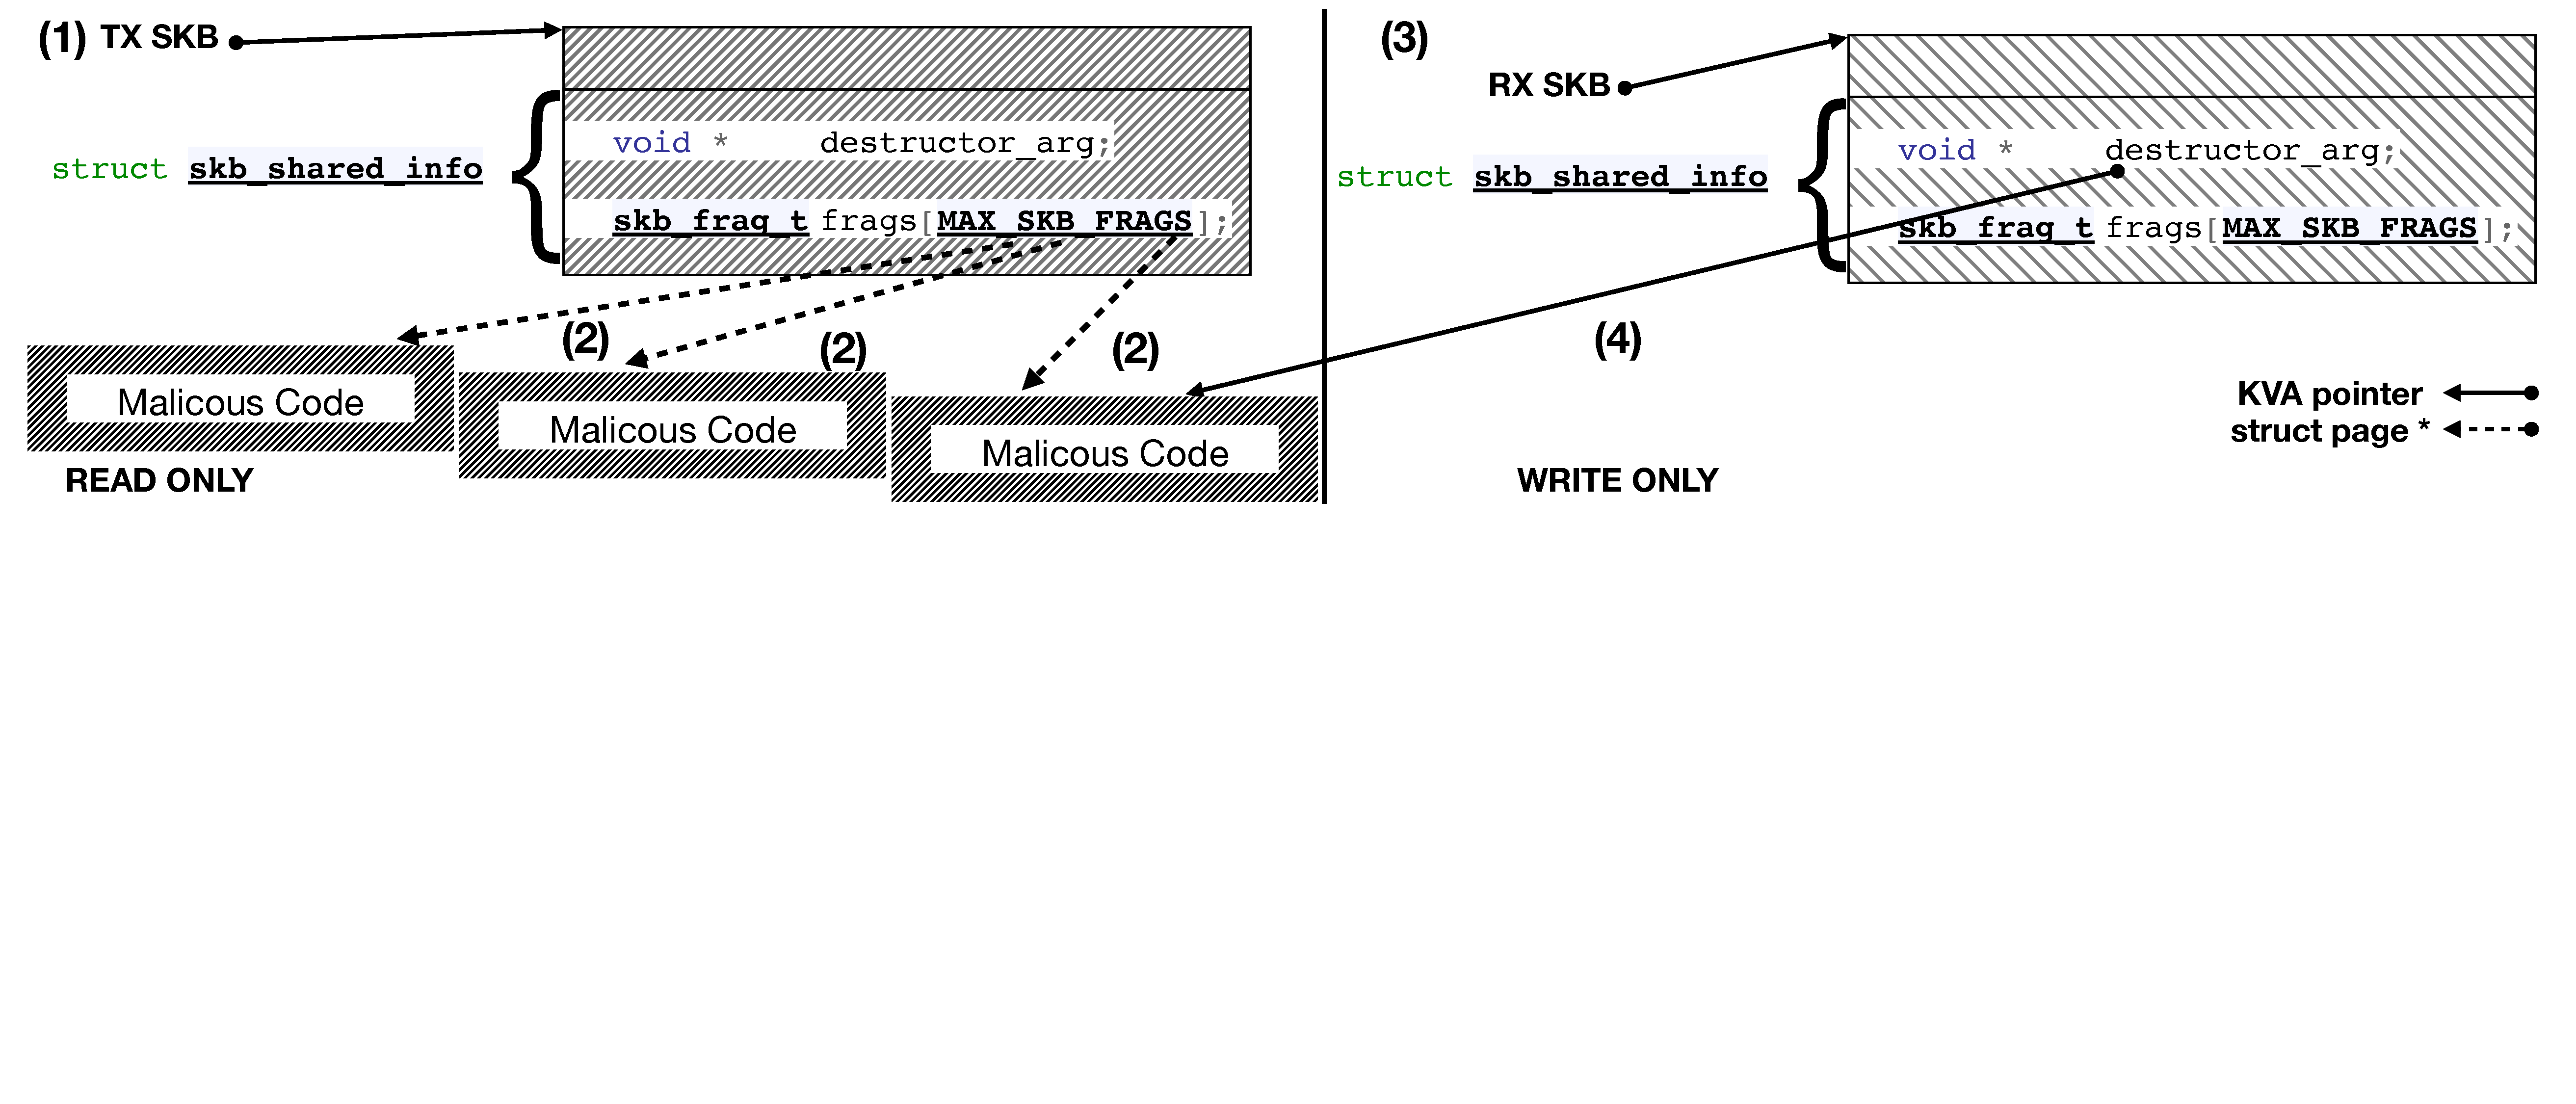
\includegraphics[width=0.8\linewidth]{figs/accomplice.pdf}
    \caption{A TX sk\_buff filled with malicious code provides the \kva for a DMA attack.}
    \label{fig:payload}
\end{figure*}
\subsection{\DIFdelbegin \DIFdel{The }\DIFdelend Poisoned TX \Compound{} Attack}\label{sec:posion}

\DIFdelbegin \DIFdel{RingFlood (Sec.~\ref{sec:ringflod}) }\DIFdelend \DIFaddbegin \DIFadd{The RingFlood attack, described in Section~\ref{sec:ringflod}, }\DIFaddend allows a NIC to execute arbitrary code\DIFdelbegin \DIFdel{with high chances of success. However, the prerequisite is sufficient }\DIFdelend \DIFaddbegin \DIFadd{, provided it has enough }\DIFaddend information regarding the server's physical layout and a sufficiently high driver memory footprint. When deducing a valid PFN is not an option (e.g., due to a low memory footprint), another way of acquiring a valid \kva{} is needed.

In this \DIFaddbegin \DIFadd{next }\DIFaddend attack, the \kva is acquired by spoofing a malicious transmitted (TX) packet. \DIFdelbegin \DIFdel{That is, the }\DIFdelend \DIFaddbegin \DIFadd{The }\DIFaddend attacker gains the needed \kva by \emph{reading} it \DIFdelbegin \DIFdel{in }\DIFdelend \DIFaddbegin \DIFadd{from }\DIFaddend the \shinfo of the sent packet. 
%
There are multiple ways in which a malicious NIC device can initiate a TX flow on the server. We list a few examples below:
\begin{enumerate}
    \item \DIFdelbegin \DIFdel{Coercing a userspace process }\DIFdelend \DIFaddbegin \DIFadd{A userspace process can be coerced }\DIFaddend into echoing a malicious buffer's contents \DIFdelbegin \DIFdel{can be achieved }\DIFdelend in various ways\DIFdelbegin \DIFdel{. For example, }\DIFdelend \DIFaddbegin \DIFadd{, including }\DIFaddend a proxy server, a key/value store\DIFdelbegin \DIFdel{and, }\DIFdelend \DIFaddbegin \DIFadd{, and }\DIFaddend a streaming service.
    \item A cloud VM (e.g., on GCP, AWS, or Azure) \DIFdelbegin \DIFdel{. A }\DIFdelend \DIFaddbegin \DIFadd{or }\DIFaddend publicly accessible VM may be used to compromise the \emph{host} in the presence of a malicious device.\footnote{Indeed, Google's OpenTitan~\cite{opentitan} exemplifies that cloud providers actively worry about the root of trust for their servers.}
    \item Packet forwarding is enabled on the server.
\end{enumerate}
%\adam{the previous sentence comes out of nowhere. add a sentence explaining the high-level idea of using a user-level process etc. The current sentence about spoofing a malicious packet isn't comprehensible.}\sout{another type of accomplice}\adam{this sounds like willingful co-operation, i.e., attacker-controlled. And that's not the intent}\SV{Rewritten. Better?} 
Since a NIC has READ access to the \shinfo{} of a TX packet, this also provides the NIC with READ access to the \texttt{frags} \DIFdelbegin \DIFdel{(Fig.~\ref{fig:payload}) }\DIFdelend array of \shinfo{}\DIFaddbegin \DIFadd{, as shown in Figure~\ref{fig:payload}}\DIFaddend . This array contains \page{} pointers \DIFdelbegin \DIFdel{, and thusboth }\DIFdelend \DIFaddbegin \DIFadd{and thus, }\DIFaddend leaks kernel pointers that allow the attacker to compromise KASLR \DIFdelbegin \DIFdel{and provides }\DIFdelend \DIFaddbegin \DIFadd{in addition to providing }\DIFaddend the PFNs of specific pages containing the data \DIFdelbegin \DIFdel{; }\DIFdelend \DIFaddbegin \DIFadd{(i.e., }\DIFaddend pages the device can read\DIFaddbegin \DIFadd{)}\DIFaddend .

%\st{Assuming an unprivileged accomplice (witing or unwitting) can open a UDP/TCP socket in user space, this user can transmit a poisoned ROP buffer. For a ROP attack (where the kernel text offset is required), the NIC spoofs an RX packet with the poisoned ROP stack to the accomplice, which in turn is sent back as a TX packet. Once an accomplice sends the packet,}
%Assuming the device can trick a userspace process into echoing a malicious buffer's contents, the device can execute a code injection attack in 4 steps:

Once the content of the malicious buffer is echoed \DIFdelbegin \DIFdel{(e.g., }\DIFdelend via one of the methods mentioned above\DIFdelbegin \DIFdel{)}\DIFdelend , the device can execute a code injection attack in \DIFdelbegin \DIFdel{4 }\DIFdelend \DIFaddbegin \DIFadd{four }\DIFaddend steps:  
%
\begin{enumerate}[labelindent=3pt]
    \item The TX \data{} and the fragments are mapped for the NIC to read.
    \item The NIC spoofs an RX packet and delays the completion notification of the TX packets \DIFdelbegin \DIFdel{(so that }\DIFdelend \DIFaddbegin \DIFadd{so }\DIFaddend the \mabaf{} \DIFdelbegin \DIFdel{will not  be released prematurely)}\DIFdelend \DIFaddbegin \DIFadd{is not  released prematurely}\DIFaddend .
    \item The NIC identifies the poisoned buffer and translates \page{} to \kva{} (\DIFdelbegin \DIFdel{Sec.}\DIFdelend \DIFaddbegin \DIFadd{Section}\DIFaddend ~\ref{sec:kaslr}).
    \item The NIC overwrites \shinfo{} with the \kva{} retrieved during step 3. 
\end{enumerate}

%\st{Tricking a userspace process into echoing a malicious buffer's contents can be archived in various ways. For example, a proxy server, a key/value store, streaming service, etc; another type of accomplice can be a cloud VM (e.g., on GCP, AWS, or Azure). A publicly accessible VM may be used to compromise the \emph{host} in the presence of a malicious device.}
%\footnote{Indeed, Googles OpenTitan~\cite{opentitan} exemplifies that cloud providers actively worry about root of trust for their servers.}

In this scenario, the attacker does not require prior knowledge regarding the physical setup since the echoed buffer provides the \kva.  

%\noindent\textbf{Timing concerns.} 
Note that an attacker will need to delay the TX completion of the echoed buffer to ensure the contents are unchanged until the ROP/JOP attack is executed.
Moreover, a TX completion event that fails to appear in due time will trigger a TX T/O error that flushes all buffers and resets the driver. The T/O is set by the driver, usually to a few seconds, \DIFaddbegin \DIFadd{which is }\DIFaddend sufficient to complete the attack.



%Namely, the only requirement for the success of this attack is an accomplice, witting (e.g., an unprivileged user) or unwitting (e.g., a proxy server) that can open a socket in user-space. For that matter, a socket in user-space of a \emph{guest machine} makes any cloud VM a valid intrusion tool in the presence of a malicious device.

%\smallskip
%\noindent\textbf{User buffer.} An attacker could try storing the \mabaf{} and code in user-space. Such and attempt would fail due to SMEP/SMAP~\cite{smep} as the kernel will not be able to directly execute user-space code.




